% !TeX root = ../main.tex

\section*{Hidden Markov Models HMM}
\paragraph{Motivation:} We want to model dependencies between features in a sequence. A HMM is a \underline{generative probabilistic approach} to describing sequential data (e.g. speech data).\\

Let \(S_1,\dots, S_N\) denote N hidden states

Let \(o_1,\dots, o_M\) denote M features (or observations, e.g. preprocessed speech data). These usually form a sequence.\\

A HMM models the joint probability (generative!) of hidden states and a sequence of observations:
\[p(<o_1,\dots, o_M>, <S_1,\dots, S_M>)\]

\paragraph{HMM Definition:} \(\lambda = (A, B, \vec{\pi})\)
\begin{itemize}
	\item A is a matrix of state transition probabilities \(a_{ij} = P[q_{t+1} = S_j | q_t = S_i]\)
	\item B is a matrix of production probabilities \(b_j(v_k) = P[v_k at state S_j]\), where \(V={v_1,\dots,v_{|V|}}\) is the set of possible observations.
	\item Values in each row of the matrices A and B sum up to 1.
	\item \(\vec{\pi}\) is a vector of starting probabilities for each state.
\end{itemize}

\begin{figure}[H]
	\centering
	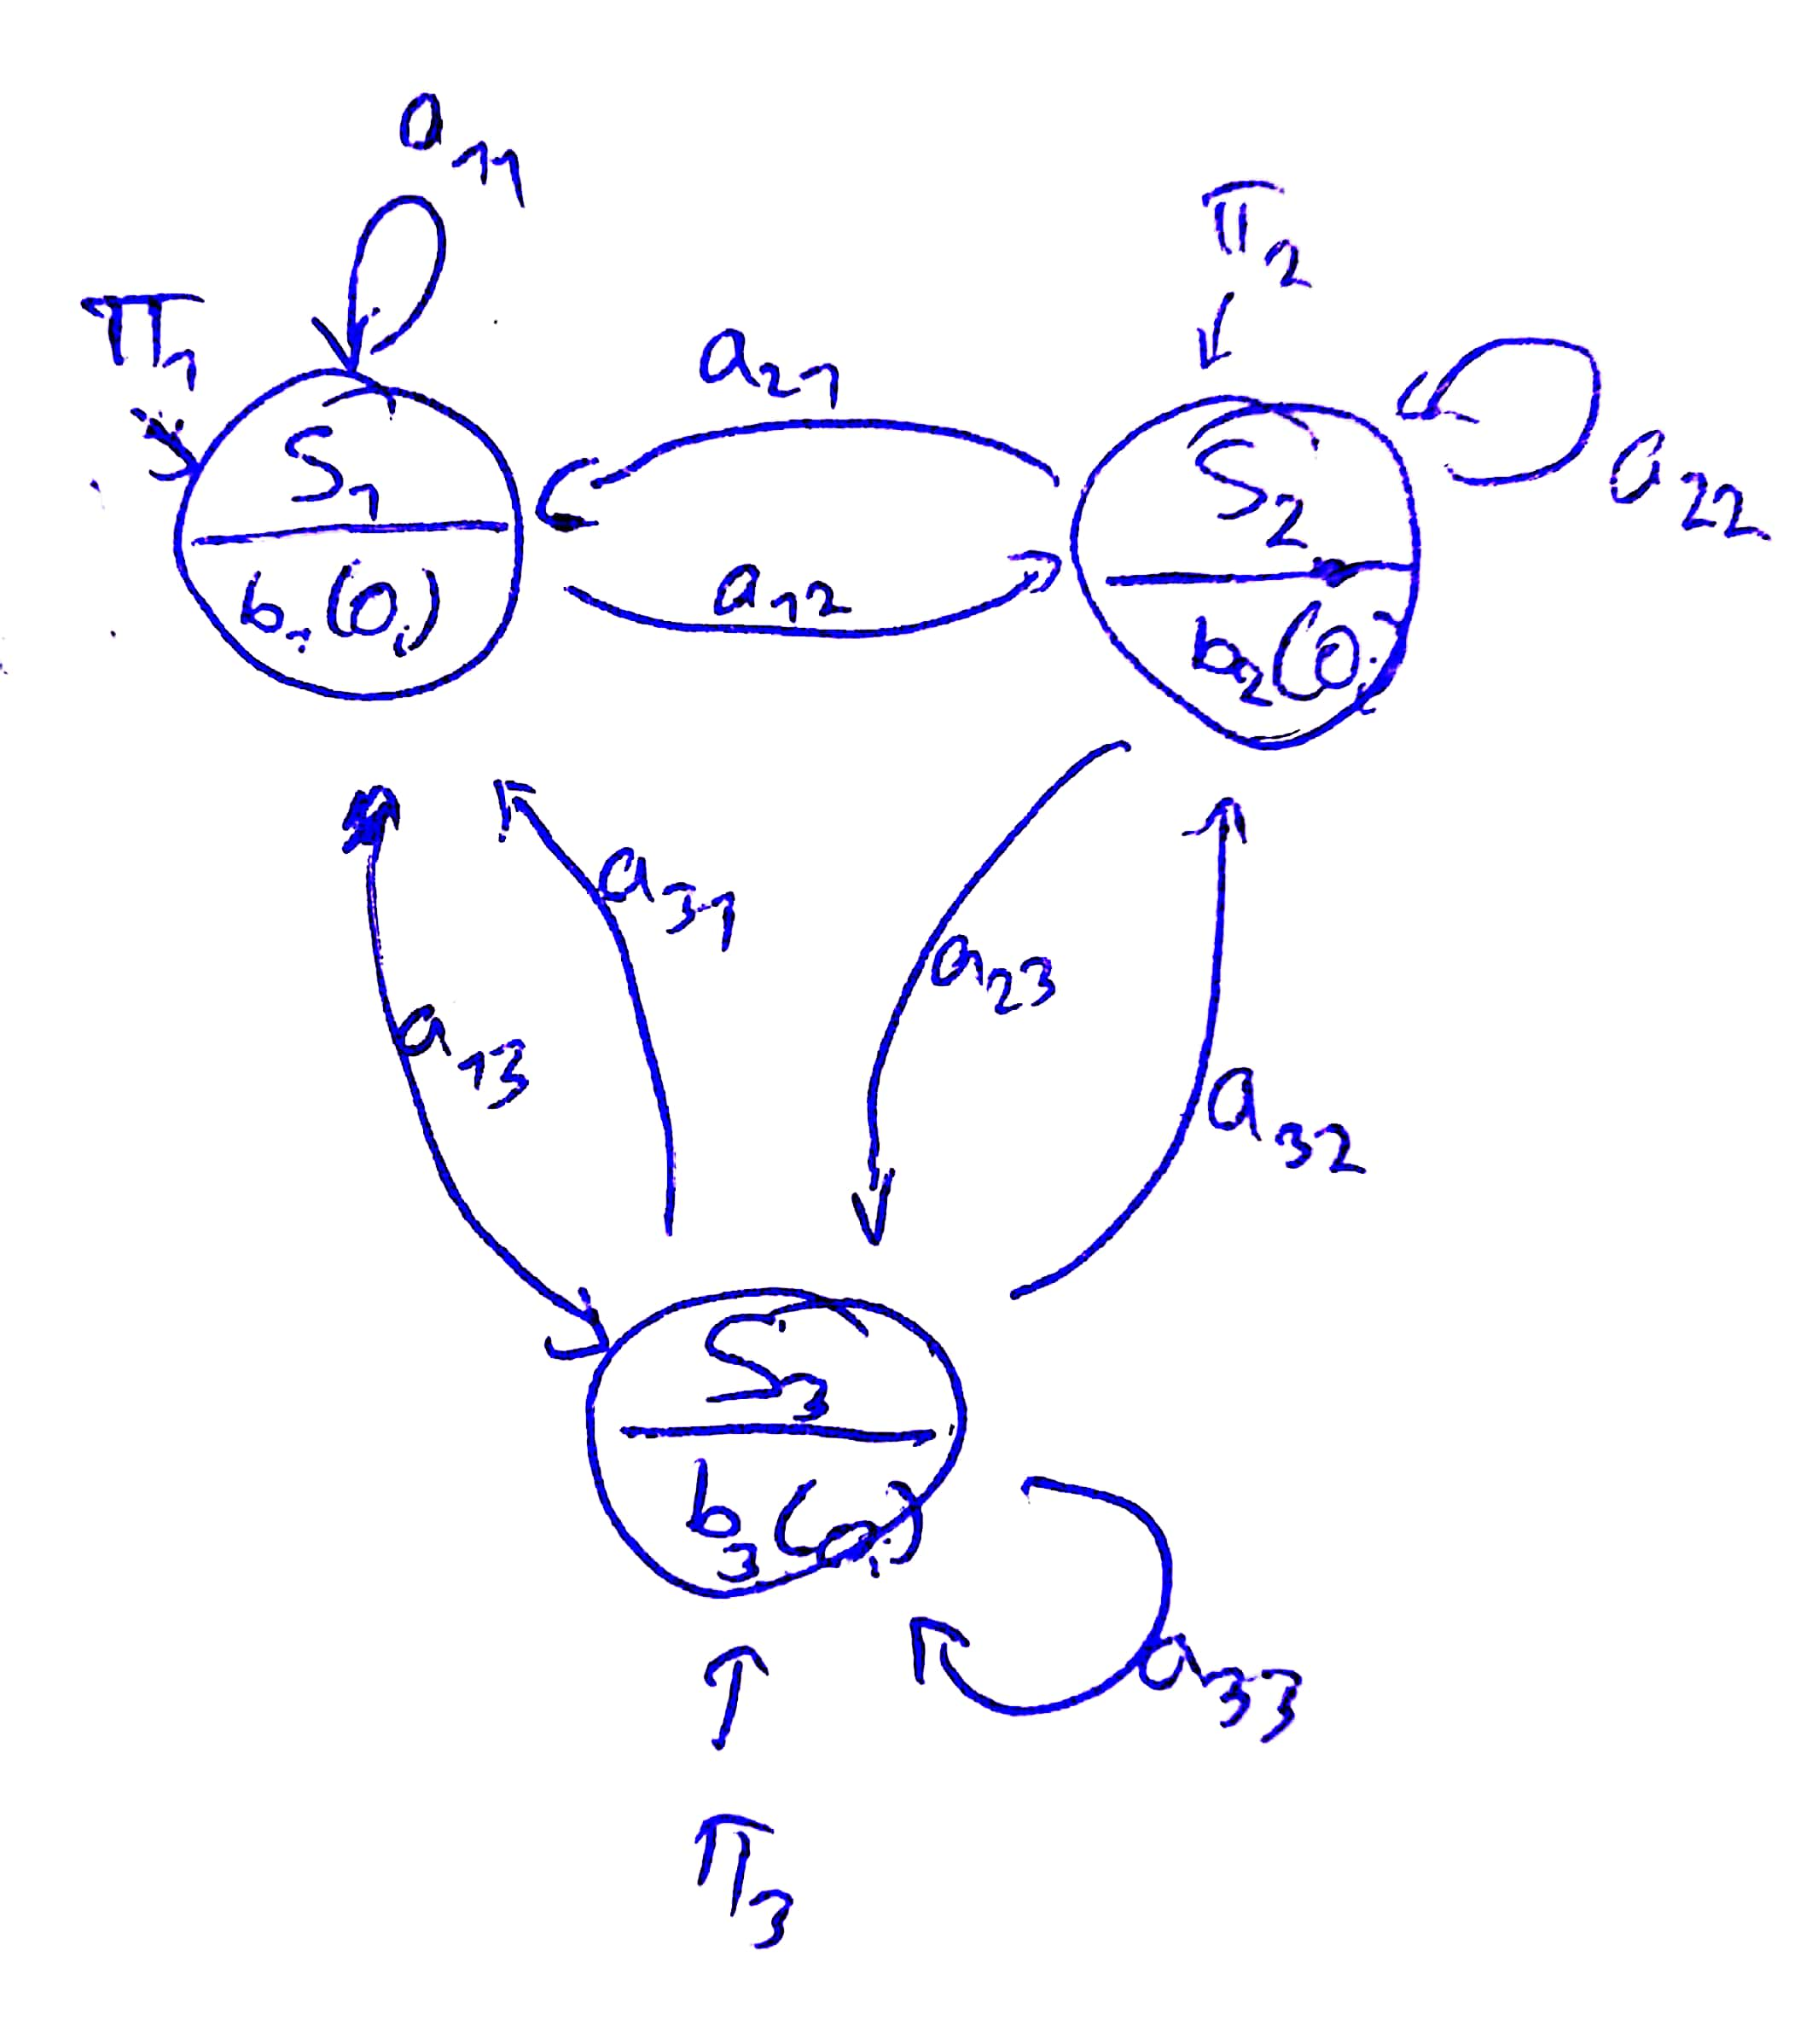
\includegraphics[width=0.4\textwidth]{hmm.jpg}
	\caption{We can represent a HMM as an graphical model similar to a state machine.}
\end{figure}

\paragraph{Questions we can ask with an HMM}

\begin{enumerate}
	\item Given a model \(\lambda\), what is \(p(<o_1,\dots, o_M>|\lambda)\), the probability of making an observation \(<o_1,\dots, o_M>\) given \(\lambda\)?
	\item Given a model \(\lambda\) and an observation sequence \(<o_1,\dots, o_M>\), what is the most likely sequence of states \(<S_1,\dots, S_M>\) that generated it?
	\item How can we obtain the model parameters \(\lambda\) in a fully automated way (training)?
\end{enumerate}

\paragraph{(1) Probability of an observation, given HMM \& known state sequence:} \emph{Forward-/Backward-Algorithm}

TODO

\paragraph{(2) Most likely state sequence} \emph{Viterbi Algorithm}

TODO

\paragraph{(3) How to train a HMM} \emph{Baum-Welch-Algorithm}

TODO

\subsection*{Remarks on HMM}

3 algorithm
\begin{enumerate}
    \item  How to train the HMM (determain the parameters $\lambda (A, B, \pi)$)
    \item  Determine the propbaility of a symbole being produced
    \item  Recover the most likly state sequence
\end{enumerate}

\begin{itemize}
    \item the directed edge in a HMM graph can be understood as a statistical dependency $p(S_2|S_1)$ (more section 8 in bishops book on pattern recognition)
    \item generative approch
    \item For many tasks including speach processing, we often only allow state transitions $a_{ij}$ with $i \le j$ (no backward links). So called "left-right-HMMs".
\end{itemize}
